\section{收敛性定理的证明}

\begin{problem}{符号函数的Fourier级数}{Sgn-Fourier-Series}
    把函数 $f(x) = \operatorname{sgn} x \ (-\uppi < x < \uppi)$ 展开为 Fourier 级数；并证明：当 $0 < x < \uppi$ 时，有 $\sum_{k=1}^{\infty} \frac{\sin(2k-1)x}{2k-1} = \frac{\uppi}{4}$，并求级数 $\sum_{n=1}^{\infty} \frac{(-1)^{n-1}}{2n-1}$．
\end{problem}

\begin{solution}
    图形如下：
    \begin{center}
        \begin{tikzpicture}[scale=0.8]
            \draw[->] (-7,0) -- (7,0) node[right] {$x$};
            \draw[->] (0,-2) -- (0,2) node[above] {$y$};

            \node[below left] at (0,0) {$0$};
            \node[below] at (3.1416,0) {$\uppi$};
            \node[below] at (-3.1416,0) {$-\uppi$};
            \node[below] at (6.2832,0) {$2\uppi$};
            \node[below] at (-6.2832,0) {$-2\uppi$};

            \draw[dashed] (-3.1416, -1.2) -- (-3.1416, 1.2);
            \draw[dashed] (3.1416, -1.2) -- (3.1416, 1.2);

            % Period -1
            \draw[thick, blue] (-6.2832, -1) -- (-3.1416, -1);
            \draw[thick, blue] (-3.1416, 1) -- (0, 1);

            % Period 0
            \draw[thick, blue] (-3.1416, -1) -- (0, -1);
            \draw[thick, blue] (0, 1) -- (3.1416, 1);

            % Period 1
            \draw[thick, blue] (3.1416, -1) -- (6.2832, -1);
            \draw[thick, blue] (6.2832, 1) -- (7, 1);

            \draw[thick, blue] (-7, -1) -- (-6.2832, -1);

            \foreach \x in {-6.2832, -3.1416, 0, 3.1416, 6.2832} {
                    \draw[fill=white, draw=blue, thick] (\x, 1) circle (2pt);
                    \draw[fill=white, draw=blue, thick] (\x, -1) circle (2pt);
                    \draw[fill=blue] (\x, 0) circle (2pt);
                }
            \node[left] at (0,1) {$1$};
            \node[left] at (0,-1) {$-1$};
        \end{tikzpicture}
    \end{center}

    由于 $f(x)$ 在区间 $(-\uppi, \uppi)$ 内是奇函数，故余弦系数为
    \begin{equation}\label{eq:sgn-an}
        a_n = 0 \quad (n = 0, 1, 2, \dots).
    \end{equation}
    正弦系数为
    \begin{equation}\label{eq:sgn-bn}
        \begin{aligned}
            b_n & = \frac{2}{\uppi} \int_{0}^{\uppi} \sin(nx) \d x        \\
                & = \left. -\frac{2}{n\uppi} \cos(nx) \right|_{0}^{\uppi} \\
                & = \frac{2(1 - (-1)^n)}{n\uppi}.
        \end{aligned}
    \end{equation}
    由此可得
    \begin{equation}\label{eq:sgn-bn-cases}
        b_{2k} = 0, \quad b_{2k-1} = \frac{4}{(2k-1)\uppi} \quad (k \in \symbb{N}^*).
    \end{equation}
    因此，函数的 Fourier 展开式为
    \begin{equation}
        \boxed{f(x) \sim \sum_{k=1}^{\infty} \frac{4}{(2k-1)\uppi} \sin(2k-1)x}.
    \end{equation}

    根据 Dirichlet 收敛定理，当 $0 < x < \uppi$ 时，函数 $f(x)$ 连续，则级数收敛于其本身，即
    \begin{equation}\label{eq:sgn-conv}
        \sum_{k=1}^{\infty} \frac{4}{(2k-1)\uppi} \sin(2k-1)x = 1.
    \end{equation}
    等式两边同乘以 $\frac{\uppi}{4}$，得
    \begin{equation}
        \boxed{\sum_{k=1}^{\infty} \frac{\sin(2k-1)x}{2k-1} = \frac{\uppi}{4}}.
    \end{equation}

    在上述等式中令 $x = \frac{\uppi}{2} \in (0, \uppi)$，代入可得
    \begin{equation}\label{eq:sub-x}
        \sum_{k=1}^{\infty} \frac{\sin(k\uppi - \frac{\uppi}{2})}{2k-1} = \sum_{k=1}^{\infty} \frac{(-1)^{k-1}}{2k-1} = \frac{\uppi}{4}.
    \end{equation}
    故所求级数之和为
    \begin{equation}
        \boxed{\sum_{n=1}^{\infty} \frac{(-1)^{n-1}}{2n-1} = \frac{\uppi}{4}}.
    \end{equation}
\end{solution}

\begin{problem}{Fourier级数展开}{Fourier-Series-Expansions}
    在区间 $(-\uppi, \uppi)$ 上把下列函数展开为 Fourier 级数：
    \begin{enumerate}
        \item $|x|$;
        \item $\sin ax \ (a \notin \symbb{Z})$;
        \item $x \sin x$.
    \end{enumerate}
\end{problem}

\begin{solution}
    \ansitem{1}

    图形如下：
    \begin{center}
        \begin{tikzpicture}[scale=0.8]
            \draw[->] (-7,0) -- (7,0) node[right] {$x$};
            \draw[->] (0,-0.5) -- (0,3.5) node[above] {$y$};

            \node[below left] at (0,0) {$0$};
            \node[below] at (3.1416,0) {$\uppi$};
            \node[below] at (-3.1416,0) {$-\uppi$};

            \draw[dashed] (-3.1416, 0) -- (-3.1416, 3.1416);
            \draw[dashed] (3.1416, 0) -- (3.1416, 3.1416);

            \draw[thick, blue] (-3.1416, 3.1416) -- (0,0) -- (3.1416, 3.1416);
            \draw[thick, blue] (3.1416, 3.1416) -- (6.2832, 0) -- (7, 0.7168);
            \draw[thick, blue] (-6.2832, 0) -- (-3.1416, 3.1416);
            \draw[thick, blue] (-7, 0.7168) -- (-6.2832, 0);

            \draw[fill=blue] (0,0) circle (2pt);
            \draw[fill=blue] (3.1416, 3.1416) circle (2pt);
            \draw[fill=blue] (-3.1416, 3.1416) circle (2pt);
            \draw[fill=blue] (6.2832, 0) circle (2pt);
            \draw[fill=blue] (-6.2832, 0) circle (2pt);
        \end{tikzpicture}
    \end{center}

    由于 $f(x) = |x|$ 在 $(-\uppi, \uppi)$ 内是偶函数，故 $b_n = 0 \ (n \geqslant 1)$．
    \begin{equation}\label{eq:abs-a0}
        a_0 = \frac{2}{\uppi} \int_{0}^{\uppi} x \d x = \uppi,
    \end{equation}
    对于 $n \geqslant 1$：
    \begin{equation}\label{eq:abs-an}
        \begin{aligned}
            a_n & = \frac{2}{\uppi} \int_{0}^{\uppi} x \cos(nx) \d x                                                                          \\
                & = \frac{2}{\uppi} \left[ \left. \frac{x \sin(nx)}{n} \right|_{0}^{\uppi} - \int_{0}^{\uppi} \frac{\sin(nx)}{n} \d x \right] \\
                & = \frac{2((-1)^n - 1)}{\uppi n^2}.
        \end{aligned}
    \end{equation}
    由此可得
    \begin{equation}\label{eq:abs-an-cases}
        a_{2k} = 0, \quad a_{2k-1} = -\frac{4}{\uppi (2k-1)^2} \quad (k \in \symbb{N}^*).
    \end{equation}
    因此，该函数的 Fourier 展开式为
    \begin{equation}
        \boxed{f(x) \sim \frac{\uppi}{2} - \sum_{k=1}^{\infty} \frac{4}{\uppi(2k-1)^2} \cos(2k-1)x}.
    \end{equation}
    收敛情况：由于周期延拓后的函数在整个实数轴上连续且分段光滑，故该级数在整个实数轴上收敛于 $f(x)$．

    \ansitem{2}

    图形如下（以 $a = 0.5$ 为例）：
    \begin{center}
        \begin{tikzpicture}[scale=0.8]
            \draw[->] (-7,0) -- (7,0) node[right] {$x$};
            \draw[->] (0,-1.5) -- (0,1.5) node[above] {$y$};

            \node[below left] at (0,0) {$0$};
            \node[below] at (3.1416,0) {$\uppi$};
            \node[below] at (-3.1416,0) {$-\uppi$};

            \draw[thick, blue, domain=-3.1416:3.1416, samples=100] plot (\x, {sin(\x/2 * 180 / 3.1416)});
            \draw[thick, blue, domain=3.1416:7, samples=100] plot (\x, {sin((\x-6.2832)/2 * 180 / 3.1416)});
            \draw[thick, blue, domain=-7:-3.1416, samples=100] plot (\x, {sin((\x+6.2832)/2 * 180 / 3.1416)});

            \draw[fill=white, draw=blue, thick] (3.1416, 1) circle (2pt);
            \draw[fill=white, draw=blue, thick] (-3.1416, -1) circle (2pt);
            \draw[fill=white, draw=blue, thick] (3.1416, -1) circle (2pt);
            \draw[fill=white, draw=blue, thick] (-3.1416, 1) circle (2pt);

            \draw[fill=blue] (3.1416, 0) circle (2pt);
            \draw[fill=blue] (-3.1416, 0) circle (2pt);
        \end{tikzpicture}
    \end{center}

    由于 $f(x) = \sin ax$ 是奇函数，故 $a_n = 0 \ (n \geqslant 0)$．
    \begin{equation}\label{eq:sinax-bn}
        \begin{aligned}
            b_n & = \frac{2}{\uppi} \int_{0}^{\uppi} \sin(ax) \sin(nx) \d x                                \\
                & = \frac{1}{\uppi} \int_{0}^{\uppi} [ \cos(a-n)x - \cos(a+n)x ] \d x                      \\
                & = \frac{1}{\uppi} \left[ \frac{\sin(a-n)\uppi}{a-n} - \frac{\sin(a+n)\uppi}{a+n} \right] \\
                & = \frac{(-1)^n \sin(a\uppi)}{\uppi} \left[ \frac{1}{a-n} - \frac{1}{a+n} \right]         \\
                & = \frac{2n (-1)^{n-1} \sin(a\uppi)}{\uppi (n^2 - a^2)}.
        \end{aligned}
    \end{equation}
    因此，该函数的 Fourier 展开式为
    \begin{equation}
        \boxed{f(x) \sim \sum_{n=1}^{\infty} \frac{2n (-1)^{n-1} \sin(a\uppi)}{\uppi (n^2 - a^2)} \sin(nx)}.
    \end{equation}
    收敛情况：由 Dirichlet 收敛定理，当 $x \in (-\uppi, \uppi)$ 时，级数收敛于 $\sin ax$；当 $x = (2k+1)\uppi \ (k \in \symbb{Z})$ 时，级数收敛于 $0$．

    \ansitem{3}

    图形如下：
    \begin{center}
        \begin{tikzpicture}[scale=0.8]
            \draw[->] (-7,0) -- (7,0) node[right] {$x$};
            \draw[->] (0,-0.5) -- (0,2.5) node[above] {$y$};

            \node[below left] at (0,0) {$0$};
            \node[below] at (3.1416,0) {$\uppi$};
            \node[below] at (-3.1416,0) {$-\uppi$};

            \draw[thick, blue, domain=-3.1416:3.1416, samples=100] plot (\x, {\x * sin(\x * 180 / 3.1416) / 3.1416});
            \draw[thick, blue, domain=3.1416:7, samples=100] plot (\x, {(\x - 6.2832) * sin((\x - 6.2832) * 180 / 3.1416) / 3.1416});
            \draw[thick, blue, domain=-7:-3.1416, samples=100] plot (\x, {(\x + 6.2832) * sin((\x + 6.2832) * 180 / 3.1416) / 3.1416});
        \end{tikzpicture}
    \end{center}

    由于 $f(x) = x \sin x$ 是偶函数，故 $b_n = 0 \ (n \geqslant 1)$．
    \begin{equation}\label{eq:xsinx-a0}
        a_0 = \frac{2}{\uppi} \int_{0}^{\uppi} x \sin x \d x = \frac{2}{\uppi} \left[ \left. -x \cos x \right|_{0}^{\uppi} + \int_{0}^{\uppi} \cos x \d x \right] = 2.
    \end{equation}
    对于 $n = 1$：
    \begin{equation}\label{eq:xsinx-a1}
        \begin{aligned}
            a_1 & = \frac{2}{\uppi} \int_{0}^{\uppi} x \sin x \cos x \d x                                                                      \\
                & = \frac{1}{\uppi} \int_{0}^{\uppi} x \sin(2x) \d x                                                                           \\
                & = \frac{1}{\uppi} \left[ \left. -\frac{x \cos(2x)}{2} \right|_{0}^{\uppi} + \int_{0}^{\uppi} \frac{\cos(2x)}{2} \d x \right] \\
                & = -\frac{1}{2}.
        \end{aligned}
    \end{equation}
    对于 $n \geqslant 2$：
    \begin{equation}\label{eq:xsinx-an}
        \begin{aligned}
            a_n & = \frac{2}{\uppi} \int_{0}^{\uppi} x \sin x \cos(nx) \d x                                                                                    \\
                & = \frac{1}{\uppi} \int_{0}^{\uppi} x [ \sin(n+1)x - \sin(n-1)x ] \d x                                                                        \\
                & = \frac{1}{\uppi} \left[ \left. -\frac{x \cos(n+1)x}{n+1} \right|_{0}^{\uppi} - \left. -\frac{x \cos(n-1)x}{n-1} \right|_{0}^{\uppi} \right] \\
                & = \frac{1}{\uppi} \left[ \frac{\uppi (-1)^n}{n+1} - \frac{\uppi (-1)^n}{n-1} \right]                                                         \\
                & = \frac{2(-1)^{n-1}}{n^2 - 1}.
        \end{aligned}
    \end{equation}
    因此，该函数的 Fourier 展开式为
    \begin{equation}
        \boxed{f(x) \sim 1 - \frac{1}{2} \cos x + \sum_{n=2}^{\infty} \frac{2(-1)^{n-1}}{n^2 - 1} \cos(nx)}.
    \end{equation}
    收敛情况：由于周期延拓后的函数在整个实数轴上连续且分段光滑，该级数在整个实数轴上收敛于 $f(x)$．
\end{solution}

\begin{problem}{分数部分函数的Fourier级数}{Fourier-Fractional-Part}
    把 $f(x) = x - [x]$（$[x]$ 是不超过 $x$ 的整数）在 $[0, 1]$ 上展开为 Fourier 级数．
\end{problem}

\begin{solution}
    图形如下：
    \begin{center}
        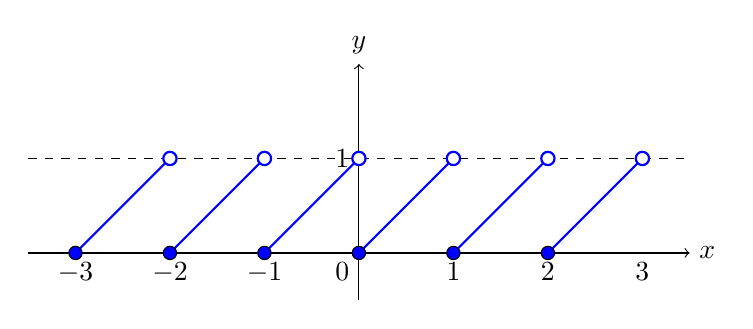
\begin{tikzpicture}[scale=1.2]
            \draw[->] (-3.5,0) -- (3.5,0) node[right] {$x$};
            \draw[->] (0,-0.5) -- (0,2) node[above] {$y$};

            \node[below left] at (0,0) {$0$};
            \node[below] at (1,0) {$1$};
            \node[below] at (2,0) {$2$};
            \node[below] at (3,0) {$3$};
            \node[below] at (-1,0) {$-1$};
            \node[below] at (-2,0) {$-2$};
            \node[below] at (-3,0) {$-3$};

            \draw[dashed] (-3.5,1) -- (3.5,1);
            \node[left] at (0,1) {$1$};

            \foreach \k in {-3,-2,-1,0,1,2} {
                    \draw[thick, blue] (\k, 0) -- (\k+1, 1);
                    \draw[fill=blue] (\k, 0) circle (2pt);
                    \draw[fill=white, draw=blue, thick] (\k+1, 1) circle (2pt);
                }
        \end{tikzpicture}
    \end{center}

    函数 $f(x) = x - [x]$ 是以 $T = 1$ 为周期的周期函数．在区间 $[0, 1)$ 上，$f(x) = x$．
    设其 Fourier 展开周期为 $2L = 1 \implies L = \frac{1}{2}$．计算其 Fourier 系数：
    \begin{equation}\label{eq:frac-a0}
        a_0 = \frac{1}{L} \int_{0}^{2L} f(x) \d x = 2 \int_{0}^{1} x \d x = 1,
    \end{equation}
    对于 $n \geqslant 1$：
    \begin{equation}\label{eq:frac-an}
        a_n = 2 \int_{0}^{1} x \cos(2n\uppi x) \d x = 2 \left[ \left. x \frac{\sin(2n\uppi x)}{2n\uppi} \right|_{0}^{1} - \int_{0}^{1} \frac{\sin(2n\uppi x)}{2n\uppi} \d x \right] = 0,
    \end{equation}
    \begin{equation}\label{eq:frac-bn}
        \begin{aligned}
            b_n & = 2 \int_{0}^{1} x \sin(2n\uppi x) \d x                                                                                          \\
                & = 2 \left[ \left. -x \frac{\cos(2n\uppi x)}{2n\uppi} \right|_{0}^{1} + \int_{0}^{1} \frac{\cos(2n\uppi x)}{2n\uppi} \d x \right] \\
                & = -\frac{1}{n\uppi}.
        \end{aligned}
    \end{equation}

    根据 Dirichlet 收敛定理，当 $x \notin \symbb{Z}$ 时，级数收敛于 $x - [x]$；当 $x \in \symbb{Z}$ 时，级数收敛于 $\frac{1}{2}$．
    因此，其 Fourier 展开式为
    \begin{equation}
        \boxed{f(x) \sim \frac{1}{2} - \sum_{n=1}^{\infty} \frac{\sin(2n\uppi x)}{n\uppi}}
    \end{equation}
\end{solution}

\begin{problem}{余弦函数的Fourier展开与三角恒等式}{Fourier-Cos-Identities}
    利用 $\cos ax$ 在 $[-\uppi, \uppi]$ 上的 Fourier 展开式，证明：
    \begin{enumerate}
        \item $\cot x = \frac{1}{x} + \sum_{n=1}^{\infty} \frac{2x}{x^2 - n^2 \uppi^2} \quad (x \neq k\uppi, \, k = 0, \pm 1, \pm 2, \dots)$;
        \item $\frac{1}{\sin x} = \frac{1}{x} + \sum_{n=1}^{\infty} (-1)^n \frac{2x}{x^2 - n^2 \uppi^2} \quad (x \neq k\uppi, \, k = 0, \pm 1, \pm 2, \dots)$.
    \end{enumerate}
\end{problem}

\begin{myproof}
    首先，我们计算 $f(y) = \cos(ay)$（$a \notin \symbb{Z}$）在 $[-\uppi, \uppi]$ 上的 Fourier 展开式．

    由于 $f(y)$ 为偶函数，所以其 Fourier 正弦系数 $b_n = 0$（$n \geqslant 1$）．
    计算余弦系数：
    \begin{equation}\label{eq:cos-a0}
        a_0 = \frac{2}{\uppi} \int_{0}^{\uppi} \cos(ay) \d y = \frac{2\sin(a\uppi)}{a\uppi},
    \end{equation}
    对于 $n \geqslant 1$：
    \begin{equation}\label{eq:cos-an}
        \begin{aligned}
            a_n & = \frac{2}{\uppi} \int_{0}^{\uppi} \cos(ay) \cos(ny) \d y                                \\
                & = \frac{1}{\uppi} \int_{0}^{\uppi} [ \cos(a+n)y + \cos(a-n)y ] \d y                      \\
                & = \frac{1}{\uppi} \left[ \frac{\sin(a+n)\uppi}{a+n} + \frac{\sin(a-n)\uppi}{a-n} \right] \\
                & = \frac{(-1)^n \sin(a\uppi)}{\uppi} \left( \frac{1}{a+n} + \frac{1}{a-n} \right)         \\
                & = \frac{2a(-1)^n \sin(a\uppi)}{\uppi (a^2 - n^2)}.
        \end{aligned}
    \end{equation}
    因为 $f(y)$ 的周期延拓在整个实数轴上连续且分段光滑，由 Dirichlet 收敛定理，对任意 $y \in [-\uppi, \uppi]$，均有以下 Fourier 展开式成立：
    \begin{equation}\label{eq:cos-expansion}
        \cos(ay) = \frac{\sin(a\uppi)}{a\uppi} + \sum_{n=1}^{\infty} \frac{2a(-1)^n \sin(a\uppi)}{\uppi (a^2 - n^2)} \cos(ny).
    \end{equation}

    \ansitem{1}

    在\zcref{eq:cos-expansion}中令 $y = \uppi$，可得
    \begin{equation}\label{eq:cot-sub}
        \cos(a\uppi) = \frac{\sin(a\uppi)}{a\uppi} + \sum_{n=1}^{\infty} \frac{2a(-1)^n \sin(a\uppi)}{\uppi (a^2 - n^2)} (-1)^n.
    \end{equation}
    由于 $(-1)^{2n} = 1$，且因为 $a \notin \symbb{Z}$，有 $\sin(a\uppi) \neq 0$，上式两边同除以 $\sin(a\uppi)$，整理得
    \begin{equation}\label{eq:cot-a}
        \cot(a\uppi) = \frac{1}{a\uppi} + \sum_{n=1}^{\infty} \frac{2a}{\uppi (a^2 - n^2)}.
    \end{equation}
    令 $x = a\uppi$（由于 $a \notin \symbb{Z}$，则 $x \neq k\uppi, \, k \in \symbb{Z}$），代入\zcref{eq:cot-a}即得
    \begin{equation}\label{eq:cot-result}
        \cot x = \frac{1}{x} + \sum_{n=1}^{\infty} \frac{2x}{x^2 - n^2 \uppi^2}.
    \end{equation}

    \ansitem{2}

    在\zcref{eq:cos-expansion}中令 $y = 0$，可得
    \begin{equation}\label{eq:sin-sub}
        1 = \frac{\sin(a\uppi)}{a\uppi} + \sum_{n=1}^{\infty} \frac{2a(-1)^n \sin(a\uppi)}{\uppi (a^2 - n^2)}.
    \end{equation}
    两边同除以 $\sin(a\uppi)$，整理得
    \begin{equation}\label{eq:csc-a}
        \frac{1}{\sin(a\uppi)} = \frac{1}{a\uppi} + \sum_{n=1}^{\infty} \frac{2a(-1)^n}{\uppi (a^2 - n^2)}.
    \end{equation}
    令 $x = a\uppi$（其中 $x \neq k\uppi, \, k \in \symbb{Z}$），代入\zcref{eq:csc-a}即得
    \begin{equation}\label{eq:csc-result}
        \frac{1}{\sin x} = \frac{1}{x} + \sum_{n=1}^{\infty} (-1)^n \frac{2x}{x^2 - n^2 \uppi^2}.
    \end{equation}
\end{myproof}

\begin{problem}{绝对值三角函数的Fourier级数}{Abs-Trig-Fourier-Series}
    证明：对任意实数 $x$，有
    \begin{enumerate}
        \item $|\cos x| = \frac{2}{\uppi} + \frac{4}{\uppi} \sum_{n=1}^{\infty} \frac{(-1)^{n-1}}{4n^2 - 1} \cos 2nx$;
        \item $|\sin x| = \frac{2}{\uppi} - \frac{4}{\uppi} \sum_{n=1}^{\infty} \frac{1}{4n^2 - 1} \cos 2nx$.
    \end{enumerate}
\end{problem}

\begin{myproof}
    \ansitem{1}

    图形如下：
    \begin{center}
        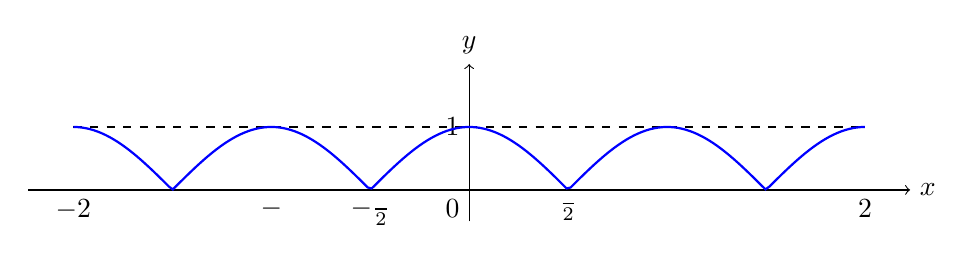
\begin{tikzpicture}[scale=0.8]
            \draw[->] (-7,0) -- (7,0) node[right] {$x$};
            \draw[->] (0,-0.5) -- (0,2) node[above] {$y$};

            \node[below left] at (0,0) {$0$};
            \node[below] at (1.5708,0) {$\frac{\uppi}{2}$};
            \node[below] at (-1.5708,0) {$-\frac{\uppi}{2}$};
            \node[below] at (3.1416,0) {$\uppi$};
            \node[below] at (-3.1416,0) {$-\uppi$};
            \node[below] at (6.2832,0) {$2\uppi$};
            \node[below] at (-6.2832,0) {$-2\uppi$};

            \draw[dashed] (0,1) -- (6.2832,1);
            \draw[dashed] (-6.2832,1) -- (0,1);
            \node[left] at (0,1) {$1$};

            \draw[thick, blue, domain=-6.2832:6.2832, samples=200] plot (\x, {abs(cos(\x*180/3.1416))});
        \end{tikzpicture}
    \end{center}

    函数 $f(x) = |\cos x|$ 是以 $\uppi$ 为周期的偶函数．在区间 $\left[-\frac{\uppi}{2}, \frac{\uppi}{2}\right]$ 上，$f(x) = \cos x$．
    设周期 $2L = \uppi \implies L = \frac{\uppi}{2}$．计算其 Fourier 系数：
    \begin{equation}\label{eq:abs-cos-a0}
        a_0 = \frac{1}{\uppi/2} \int_{-\uppi/2}^{\uppi/2} \cos x \d x = \frac{4}{\uppi},
    \end{equation}
    对于 $n \geqslant 1$：
    \begin{equation}\label{eq:abs-cos-an}
        \begin{aligned}
            a_n & = \frac{1}{\uppi/2} \int_{-\uppi/2}^{\uppi/2} \cos x \cos(2nx) \d x                                               \\
                & = \frac{1}{\uppi} \int_{-\uppi/2}^{\uppi/2} [\cos(2n+1)x + \cos(2n-1)x] \d x                                      \\
                & = \frac{1}{\uppi} \left[ \frac{\sin(2n+1)x}{2n+1} + \frac{\sin(2n-1)x}{2n-1} \right]_{-\uppi/2}^{\uppi/2}         \\
                & = \frac{2}{\uppi} \left[ \frac{\sin(2n+1)\frac{\uppi}{2}}{2n+1} + \frac{\sin(2n-1)\frac{\uppi}{2}}{2n-1} \right].
        \end{aligned}
    \end{equation}
    注意到 $\sin(2n+1)\frac{\uppi}{2} = (-1)^n$，且 $\sin(2n-1)\frac{\uppi}{2} = (-1)^{n-1}$，代入\zcref{eq:abs-cos-an}得
    \begin{equation}\label{eq:abs-cos-an-result}
        \begin{aligned}
            a_n & = \frac{2}{\uppi} \left[ \frac{(-1)^n}{2n+1} + \frac{(-1)^{n-1}}{2n-1} \right] \\
                & = \frac{2(-1)^{n-1}}{\uppi} \left( \frac{1}{2n-1} - \frac{1}{2n+1} \right)     \\
                & = \frac{4(-1)^{n-1}}{\uppi(4n^2 - 1)}.
        \end{aligned}
    \end{equation}
    由于 $f(x)$ 在整个实数轴上连续且分段光滑，由 Dirichlet 收敛定理，级数在整个实数轴上收敛于 $f(x)$，故有
    \begin{equation}
        \boxed{|\cos x| = \frac{2}{\uppi} + \frac{4}{\uppi} \sum_{n=1}^{\infty} \frac{(-1)^{n-1}}{4n^2 - 1} \cos 2nx}
    \end{equation}

    \ansitem{2}

    图形如下：
    \begin{center}
        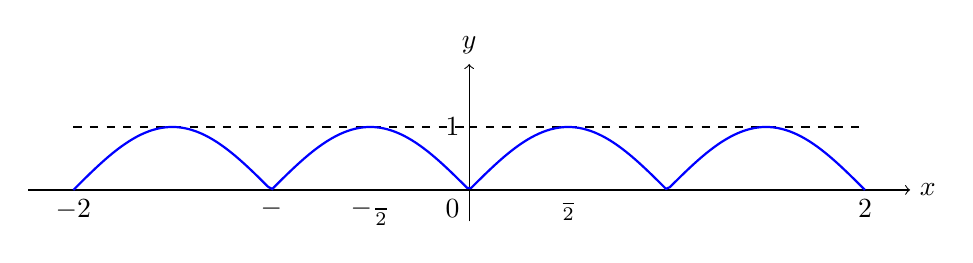
\begin{tikzpicture}[scale=0.8]
            \draw[->] (-7,0) -- (7,0) node[right] {$x$};
            \draw[->] (0,-0.5) -- (0,2) node[above] {$y$};

            \node[below left] at (0,0) {$0$};
            \node[below] at (1.5708,0) {$\frac{\uppi}{2}$};
            \node[below] at (-1.5708,0) {$-\frac{\uppi}{2}$};
            \node[below] at (3.1416,0) {$\uppi$};
            \node[below] at (-3.1416,0) {$-\uppi$};
            \node[below] at (6.2832,0) {$2\uppi$};
            \node[below] at (-6.2832,0) {$-2\uppi$};

            \draw[dashed] (0,1) -- (6.2832,1);
            \draw[dashed] (-6.2832,1) -- (0,1);
            \node[left] at (0,1) {$1$};

            \draw[thick, blue, domain=-6.2832:6.2832, samples=200] plot (\x, {abs(sin(\x*180/3.1416))});
        \end{tikzpicture}
    \end{center}

    利用恒等式 $|\sin x| = \left| \cos\left( x - \frac{\uppi}{2} \right) \right|$，将第一问结论中的 $x$ 替换为 $x - \frac{\uppi}{2}$，得
    \begin{equation}\label{eq:abs-sin-sub}
        |\sin x| = \frac{2}{\uppi} + \frac{4}{\uppi} \sum_{n=1}^{\infty} \frac{(-1)^{n-1}}{4n^2 - 1} \cos\left[ 2n\left( x - \frac{\uppi}{2} \right) \right].
    \end{equation}
    因为对任意整数 $n$ 有
    \begin{equation}\label{eq:cos-shift-identity}
        \cos(2nx - n\uppi) = (-1)^n \cos 2nx,
    \end{equation}
    所以\zcref{eq:abs-sin-sub}中的通项化简为
    \begin{equation}\label{eq:abs-sin-term}
        (-1)^{n-1} \cos\left[ 2n\left( x - \frac{\uppi}{2} \right) \right] = (-1)^{n-1}(-1)^n \cos 2nx = -\cos 2nx.
    \end{equation}
    代入\zcref{eq:abs-sin-sub}后，即证得
    \begin{equation}
        \boxed{|\sin x| = \frac{2}{\uppi} - \frac{4}{\uppi} \sum_{n=1}^{\infty} \frac{1}{4n^2 - 1} \cos 2nx}
    \end{equation}
\end{myproof}

\begin{problem}{指数函数的Fourier展开}{Exponential-Fourier-Series}
    对 $x \in (0, 2\uppi)$ 以及 $a \neq 0$，求证：
    \begin{equation*}
        \e^{ax} = \frac{\e^{2a\uppi} - 1}{\uppi} \left( \frac{1}{2a} + \sum_{k=1}^{\infty} \frac{a \cos kx - k \sin kx}{k^2 + a^2} \right).
    \end{equation*}
\end{problem}

\begin{myproof}
    图形如下：
    \begin{center}
        \begin{tikzpicture}[xscale=0.8, yscale=0.8]
            \draw[->] (-7,0) -- (7,0) node[right] {$x$};
            \draw[->] (0,-0.5) -- (0,5.5) node[above] {$y$};
            \node[below left] at (0,0) {$0$};
            \node[below] at (3.1416,0) {$\uppi$};
            \node[below] at (6.2832,0) {$2\uppi$};
            \node[below] at (-3.1416,0) {$-\uppi$};
            \node[below] at (-6.2832,0) {$-2\uppi$};

            % Period -1: [-2pi, 0)
            \draw[thick, blue, domain=-6.2832:-0.05, samples=100] plot (\x, {exp(0.25*(\x+6.2832))});
            \draw[fill=blue] (-6.2832, 1) circle (2pt);
            \draw[fill=white, draw=blue, thick] (0, {exp(0.25*6.2832)}) circle (2pt);

            % Period 0: [0, 2pi)
            \draw[thick, blue, domain=0:6.2332, samples=100] plot (\x, {exp(0.25*\x)});
            \draw[fill=blue] (0, 1) circle (2pt);
            \draw[fill=white, draw=blue, thick] (6.2832, {exp(0.25*6.2832)}) circle (2pt);

            % Period 1: [2pi, 4pi)
            \draw[thick, blue, domain=6.2832:7, samples=50] plot (\x, {exp(0.25*(\x-6.2832))});
            \draw[fill=blue] (6.2832, 1) circle (2pt);

            % Period -2: left edge
            \draw[thick, blue, domain=-7:-6.2832, samples=50] plot (\x, {exp(0.25*(\x+12.5664))});
            \draw[fill=white, draw=blue, thick] (-6.2832, {exp(0.25*6.2832)}) circle (2pt);

            % Midpoints for convergence at discontinuities
            \foreach \x in {-6.2832, 0, 6.2832} {
                    \draw[fill=red] (\x, {(1 + exp(0.25*6.2832))/2}) circle (2pt);
                }

            \node[left] at (0,1) {$1$};
            \node[left] at (0,4.81) {$\e^{2a\uppi}$};
            \draw[dashed] (0,4.81) -- (6.2832, 4.81);
        \end{tikzpicture}
    \end{center}

    设函数 $f(x) = \e^{ax}$ 在 $(0, 2\uppi)$ 上的周期延拓周期为 $2L = 2\uppi \implies L = \uppi$．计算其 Fourier 系数：
    \begin{equation}\label{eq:exp-a0-val}
        a_0 = \frac{1}{\uppi} \int_{0}^{2\uppi} \e^{ax} \d x = \frac{\e^{2a\uppi} - 1}{a\uppi},
    \end{equation}
    对于 $k \geqslant 1$，利用分部积分得
    \begin{equation}\label{eq:exp-ak-val}
        \begin{aligned}
            a_k & = \frac{1}{\uppi} \int_{0}^{2\uppi} \e^{ax} \cos(kx) \d x                                      \\
                & = \frac{1}{\uppi} \left. \frac{\e^{ax}(a \cos kx + k \sin kx)}{k^2 + a^2} \right|_{0}^{2\uppi} \\
                & = \frac{\e^{2a\uppi} - 1}{\uppi} \frac{a}{k^2 + a^2},
        \end{aligned}
    \end{equation}
    以及
    \begin{equation}\label{eq:exp-bk-val}
        \begin{aligned}
            b_k & = \frac{1}{\uppi} \int_{0}^{2\uppi} \e^{ax} \sin(kx) \d x                                      \\
                & = \frac{1}{\uppi} \left. \frac{\e^{ax}(a \sin kx - k \cos kx)}{k^2 + a^2} \right|_{0}^{2\uppi} \\
                & = -\frac{\e^{2a\uppi} - 1}{\uppi} \frac{k}{k^2 + a^2}.
        \end{aligned}
    \end{equation}
    由于 $f(x) = \e^{ax}$ 在开区间 $(0, 2\uppi)$ 内连续且可微，由 Dirichlet 收敛定理，在此开区间内级数收敛于自身：
    \begin{equation}\label{eq:exp-sum}
        \begin{aligned}
            \e^{ax} & = \frac{a_0}{2} + \sum_{k=1}^{\infty} (a_k \cos kx + b_k \sin kx)                                                                                                                               \\
                    & = \frac{\e^{2a\uppi} - 1}{2a\uppi} + \sum_{k=1}^{\infty} \left[ \frac{\e^{2a\uppi} - 1}{\uppi} \frac{a \cos kx}{k^2 + a^2} - \frac{\e^{2a\uppi} - 1}{\uppi} \frac{k \sin kx}{k^2 + a^2} \right] \\
                    & = \frac{\e^{2a\uppi} - 1}{\uppi} \left( \frac{1}{2a} + \sum_{k=1}^{\infty} \frac{a \cos kx - k \sin kx}{k^2 + a^2} \right).
        \end{aligned}
    \end{equation}
    故对 $x \in (0, 2\uppi)$，有
    \begin{equation}
        \boxed{\e^{ax} = \frac{\e^{2a\uppi} - 1}{\uppi} \left( \frac{1}{2a} + \sum_{k=1}^{\infty} \frac{a \cos kx - k \sin kx}{k^2 + a^2} \right)}
    \end{equation}
\end{myproof}

\begin{problem}{Fourier级数逐项积分}{Fourier-Term-by-Term-Integration}
    对展开式
    \begin{equation}\label{eq:base-fourier}
        x = 2 \sum_{n=1}^{\infty} (-1)^{n-1} \frac{\sin nx}{n} \quad (-\uppi < x < \uppi)
    \end{equation}
    逐项积分，求函数 $x^2$、 $x^3$ 和 $x^4$ 在区间 $(-\uppi, \uppi)$ 上的 Fourier 展开式，并证明：
    \begin{equation*}
        \sum_{n=1}^{\infty} \frac{1}{n^6} = \frac{\uppi^6}{945}, \quad \sum_{n=1}^{\infty} \frac{1}{n^8} = \frac{\uppi^8}{9450}.
    \end{equation*}
\end{problem}

\begin{solution}
    图形如下（以 $y=x^2$ 和 $y=x^3$ 的周期延拓为例）：
    \begin{center}
        \begin{tikzpicture}[scale=0.6]
            \draw[->] (-7,0) -- (7,0) node[right] {$x$};
            \draw[->] (0,-0.5) -- (0,4) node[above] {$y$};
            \node[below left] at (0,0) {$0$};
            \node[below] at (3.1416,0) {$\uppi$};
            \node[below] at (-3.1416,0) {$-\uppi$};
            \draw[dashed] (-3.1416,0) -- (-3.1416,3.1416);
            \draw[dashed] (3.1416,0) -- (3.1416,3.1416);
            \draw[thick, blue, domain=-3.1416:3.1416, samples=100] plot (\x, {\x*\x/3.1416});
            \draw[thick, blue, domain=3.1416:6.2832, samples=100] plot (\x, {(\x-6.2832)*(\x-6.2832)/3.1416});
            \draw[thick, blue, domain=-6.2832:-3.1416, samples=100] plot (\x, {(\x+6.2832)*(\x+6.2832)/3.1416});
            \draw[fill=blue] (3.1416, 3.1416) circle (2pt);
            \draw[fill=blue] (-3.1416, 3.1416) circle (2pt);
            \node[left] at (0, 3.1416) {$\uppi^2$};
            \node[above] at (0, -1.8) {$y = x^2$ 的周期延拓};
        \end{tikzpicture}
        \quad
        \begin{tikzpicture}[scale=0.6]
            \draw[->] (-7,0) -- (7,0) node[right] {$x$};
            \draw[->] (0,-4) -- (0,4) node[above] {$y$};
            \node[below left] at (0,0) {$0$};
            \node[below] at (3.1416,0) {$\uppi$};
            \node[below] at (-3.1416,0) {$-\uppi$};
            \draw[dashed] (-3.1416,-3.1416) -- (-3.1416,3.1416);
            \draw[dashed] (3.1416,-3.1416) -- (3.1416,3.1416);
            \draw[thick, blue, domain=-3.1416:3.1416, samples=100] plot (\x, {\x*\x*\x/9.8696});
            \draw[thick, blue, domain=3.1416:6.2832, samples=100] plot (\x, {(\x-6.2832)*(\x-6.2832)*(\x-6.2832)/9.8696});
            \draw[thick, blue, domain=-6.2832:-3.1416, samples=100] plot (\x, {(\x+6.2832)*(\x+6.2832)*(\x+6.2832)/9.8696});
            \draw[fill=white, draw=blue, thick] (3.1416, 3.1416) circle (2pt);
            \draw[fill=white, draw=blue, thick] (-3.1416, -3.1416) circle (2pt);
            \draw[fill=white, draw=blue, thick] (3.1416, -3.1416) circle (2pt);
            \draw[fill=white, draw=blue, thick] (-3.1416, 3.1416) circle (2pt);
            \draw[fill=blue] (3.1416, 0) circle (2pt);
            \draw[fill=blue] (-3.1416, 0) circle (2pt);
            \node[left] at (0, 3.1416) {$\uppi^3$};
            \node[left] at (0, -3.1416) {$-\uppi^3$};
            \node[above] at (0, -5) {$y = x^3$ 的周期延拓};
        \end{tikzpicture}
    \end{center}

    \ansitem{1}

    对\zcref{eq:base-fourier}在区间 $[0, x]$ 上逐项积分，其中 $-\uppi < x < \uppi$：
    \begin{equation}\label{eq:int-x2}
        \frac{x^2}{2} = 2 \sum_{n=1}^{\infty} \frac{(-1)^{n-1}}{n} \int_{0}^{x} \sin nt \d t = 2 \sum_{n=1}^{\infty} \frac{(-1)^{n-1}}{n^2} (1 - \cos nx).
    \end{equation}
    由于交错级数恒等式：
    \begin{equation}\label{eq:eta2}
        \sum_{n=1}^{\infty} \frac{(-1)^{n-1}}{n^2} = \frac{\uppi^2}{12},
    \end{equation}
    代入\zcref{eq:int-x2}可得
    \begin{equation}\label{eq:x2-half}
        \frac{x^2}{2} = \frac{\uppi^2}{6} + 2 \sum_{n=1}^{\infty} \frac{(-1)^n}{n^2} \cos nx.
    \end{equation}
    两边同乘以 $2$，即得 $x^2$ 的 Fourier 展开式：
    \begin{equation}
        \boxed{x^2 = \frac{\uppi^2}{3} + 4 \sum_{n=1}^{\infty} \frac{(-1)^n}{n^2} \cos nx}
    \end{equation}

    \ansitem{2}

    对\zcref{eq:x2-half}再次在 $[0, x]$ 上逐项积分，得
    \begin{equation}\label{eq:int-x3}
        \frac{x^3}{6} = \frac{\uppi^2 x}{6} + 2 \sum_{n=1}^{\infty} \frac{(-1)^n}{n^3} \sin nx.
    \end{equation}
    将\zcref{eq:base-fourier}代入\zcref{eq:int-x3}中的第一项，有
    \begin{equation}\label{eq:sub-x3}
        \frac{x^3}{6} = \frac{\uppi^2}{3} \sum_{n=1}^{\infty} \frac{(-1)^{n-1}}{n} \sin nx - 2 \sum_{n=1}^{\infty} \frac{(-1)^{n-1}}{n^3} \sin nx.
    \end{equation}
    整理并两边同乘以 $6$，即得 $x^3$ 的 Fourier 展开式：
    \begin{equation}
        \boxed{x^3 = 2 \sum_{n=1}^{\infty} (-1)^{n-1} \left( \frac{\uppi^2}{n} - \frac{6}{n^3} \right) \sin nx}
    \end{equation}

    \ansitem{3}

    对\zcref{eq:sub-x3}继续在 $[0, x]$ 上逐项积分，得
    \begin{equation}\label{eq:int-x4}
        \frac{x^4}{24} = \sum_{n=1}^{\infty} (-1)^{n-1} \left( \frac{\uppi^2}{3n^2} - \frac{2}{n^4} \right) (1 - \cos nx).
    \end{equation}
    已知下列交错级数和：
    \begin{equation}\label{eq:eta2-4}
        \sum_{n=1}^{\infty} \frac{(-1)^{n-1}}{n^2} = \frac{\uppi^2}{12}, \quad \sum_{n=1}^{\infty} \frac{(-1)^{n-1}}{n^4} = \frac{7\uppi^4}{720}.
    \end{equation}
    计算常数项：
    \begin{equation}\label{eq:const-x4}
        C = \sum_{n=1}^{\infty} (-1)^{n-1} \left( \frac{\uppi^2}{3n^2} - \frac{2}{n^4} \right) = \frac{\uppi^2}{3} \left( \frac{\uppi^2}{12} \right) - 2 \left( \frac{7\uppi^4}{720} \right) = \frac{\uppi^4}{120}.
    \end{equation}
    将其代入\zcref{eq:int-x4}中，可得
    \begin{equation}\label{eq:x4-fraction}
        \frac{x^4}{24} = \frac{\uppi^4}{120} + \sum_{n=1}^{\infty} (-1)^n \left( \frac{\uppi^2}{3n^2} - \frac{2}{n^4} \right) \cos nx.
    \end{equation}
    两边同乘以 $24$，即得 $x^4$ 的 Fourier 展开式：
    \begin{equation}
        \boxed{x^4 = \frac{\uppi^4}{5} + 8 \sum_{n=1}^{\infty} (-1)^n \left( \frac{\uppi^2}{n^2} - \frac{6}{n^4} \right) \cos nx}
    \end{equation}

    \ansitem{4}

    利用 Parseval 等式进行级数求和．

    首先，对 $x^3$ 的 Fourier 展开式应用 Parseval 等式：
    \begin{equation}\label{eq:parseval-x3}
        \frac{1}{\uppi} \int_{-\uppi}^{\uppi} (x^3)^2 \d x = \sum_{n=1}^{\infty} b_n^2,
    \end{equation}
    即
    \begin{equation}\label{eq:parseval-x3-calc}
        \frac{2\uppi^6}{7} = 4 \sum_{n=1}^{\infty} \left( \frac{\uppi^4}{n^2} - \frac{12\uppi^2}{n^4} + \frac{36}{n^6} \right).
    \end{equation}
    代入已知值 $\sum_{n=1}^{\infty} \frac{1}{n^2} = \frac{\uppi^2}{6}$ 和 $\sum_{n=1}^{\infty} \frac{1}{n^4} = \frac{\uppi^4}{90}$，有
    \begin{equation}\label{eq:parseval-x3-subs}
        \frac{\uppi^6}{14} = \frac{\uppi^6}{6} - \frac{2\uppi^6}{15} + 36 \sum_{n=1}^{\infty} \frac{1}{n^6} = \frac{\uppi^6}{30} + 36 \sum_{n=1}^{\infty} \frac{1}{n^6}.
    \end{equation}
    由此解得第一个级数的和：
    \begin{equation}
        \boxed{\sum_{n=1}^{\infty} \frac{1}{n^6} = \frac{\uppi^6}{945}}
    \end{equation}

    其次，对 $x^4$ 的 Fourier 展开式应用 Parseval 等式：
    \begin{equation}\label{eq:parseval-x4}
        \frac{1}{\uppi} \int_{-\uppi}^{\uppi} (x^4)^2 \d x = \frac{a_0^2}{2} + \sum_{n=1}^{\infty} a_n^2,
    \end{equation}
    其中 $\frac{a_0}{2} = \frac{\uppi^4}{5} \implies a_0 = \frac{2\uppi^4}{5}$，代入得
    \begin{equation}\label{eq:parseval-x4-calc}
        \frac{2\uppi^8}{9} = \frac{2\uppi^8}{25} + 64 \sum_{n=1}^{\infty} \left( \frac{\uppi^4}{n^4} - \frac{12\uppi^2}{n^6} + \frac{36}{n^8} \right).
    \end{equation}
    移项并整理得
    \begin{equation}\label{eq:parseval-x4-subs}
        \frac{\uppi^8}{450} = \uppi^4 \sum_{n=1}^{\infty} \frac{1}{n^4} - 12\uppi^2 \sum_{n=1}^{\infty} \frac{1}{n^6} + 36 \sum_{n=1}^{\infty} \frac{1}{n^8}.
    \end{equation}
    代入已知值 $\sum_{n=1}^{\infty} \frac{1}{n^4} = \frac{\uppi^4}{90}$ 和上一步得到的 $\sum_{n=1}^{\infty} \frac{1}{n^6} = \frac{\uppi^6}{945}$：
    \begin{equation}\label{eq:parseval-x4-final}
        \frac{\uppi^8}{450} = \frac{\uppi^8}{90} - \frac{4\uppi^8}{315} + 36 \sum_{n=1}^{\infty} \frac{1}{n^8}.
    \end{equation}
    移项通分计算得
    \begin{equation}\label{eq:final-sum-8}
        36 \sum_{n=1}^{\infty} \frac{1}{n^8} = \uppi^8 \left( \frac{1}{450} + \frac{4}{315} - \frac{1}{90} \right) = \frac{12\uppi^8}{3150}.
    \end{equation}
    由此解得第二个级数的和：
    \begin{equation}
        \boxed{\sum_{n=1}^{\infty} \frac{1}{n^8} = \frac{\uppi^8}{9450}}
    \end{equation}
\end{solution}

\begin{problem}{分段函数的正弦级数展开}{Segmented-Sine-Series}
    设 $f(x) = \begin{cases} \frac{\uppi-1}{2}x, & 0 \leqslant x \leqslant 1, \\ \frac{\uppi-x}{2}, & 1 < x \leqslant \uppi \end{cases}$，证明：
    \begin{equation*}
        f(x) = \sum_{n=1}^{\infty} \frac{\sin n}{n^2} \sin nx \quad (0 \leqslant x \leqslant \uppi).
    \end{equation*}
\end{problem}

\begin{myproof}
    图形如下：
    \begin{center}
        \begin{tikzpicture}[scale=1.2]
            \draw[->] (-4,0) -- (4,0) node[right] {$x$};
            \draw[->] (0,-1.5) -- (0,1.5) node[above] {$y$};

            \node[below left] at (0,0) {$0$};
            \node[below] at (3.1416,0) {$\uppi$};
            \node[below] at (-3.1416,0) {$-\uppi$};
            \node[below] at (1,0) {$1$};
            \node[below] at (-1,0) {$-1$};

            \draw[dashed] (1,0) -- (1,1.07);
            \draw[dashed] (0,1.07) -- (1,1.07);
            \node[left] at (0,1.07) {$\frac{\uppi-1}{2}$};

            \draw[thick, blue] (-3.1416, 0) -- (-1, -1.07) -- (0,0) -- (1, 1.07) -- (3.1416, 0);

            \draw[fill=blue] (0,0) circle (2pt);
            \draw[fill=blue] (3.1416, 0) circle (2pt);
            \draw[fill=blue] (-3.1416, 0) circle (2pt);
            \draw[fill=blue] (1, 1.07) circle (2pt);
            \draw[fill=blue] (-1, -1.07) circle (2pt);
        \end{tikzpicture}
    \end{center}

    为了将 $f(x)$ 展开为正弦级数，将其作奇延拓到 $[-\uppi, \uppi]$ 上．其 Fourier 系数满足 $a_n = 0 \ (n \geqslant 0)$，正弦系数为
    \begin{equation}\label{eq:sine-bn-integral}
        b_n = \frac{2}{\uppi} \int_{0}^{\uppi} f(x) \sin nx \d x.
    \end{equation}
    将 $f(x)$ 的分段表达式代入\zcref{eq:sine-bn-integral}中，可得
    \begin{equation}\label{eq:sine-bn-calc}
        b_n = \frac{2}{\uppi} \left[ \int_{0}^{1} \frac{\uppi-1}{2} x \sin nx \d x + \int_{1}^{\uppi} \frac{\uppi-x}{2} \sin nx \d x \right].
    \end{equation}
    分别计算两个积分项．第一项为
    \begin{equation}\label{eq:sine-part1}
        \int_{0}^{1} x \sin nx \d x = \left. -x \frac{\cos nx}{n} \right|_{0}^{1} + \int_{0}^{1} \frac{\cos nx}{n} \d x = -\frac{\cos n}{n} + \frac{\sin n}{n^2},
    \end{equation}
    第二项为
    \begin{equation}\label{eq:sine-part2}
        \int_{1}^{\uppi} (\uppi-x) \sin nx \d x = \left. -(\uppi-x) \frac{\cos nx}{n} \right|_{1}^{\uppi} - \int_{1}^{\uppi} \frac{\cos nx}{n} \d x = \frac{(\uppi-1)\cos n}{n} + \frac{\sin n}{n^2}.
    \end{equation}
    将\zcref{eq:sine-part1}与\zcref{eq:sine-part2}代入\zcref{eq:sine-bn-calc}，合并同类项整理得
    \begin{equation}\label{eq:sine-bn-final}
        \begin{aligned}
            b_n & = \frac{1}{\uppi} \left[ (\uppi-1) \left( -\frac{\cos n}{n} + \frac{\sin n}{n^2} \right) + \left( \frac{(\uppi-1)\cos n}{n} + \frac{\sin n}{n^2} \right) \right] \\
                & = \frac{1}{\uppi} \left[ \uppi \frac{\sin n}{n^2} \right] = \frac{\sin n}{n^2}.
        \end{aligned}
    \end{equation}
    由于 $f(x)$ 在整个区间 $[0, \uppi]$ 上连续且分段光滑，由 Dirichlet 收敛定理，该 Fourier 级数在 $[0, \uppi]$ 上处处收敛于 $f(x)$ 本身，即有
    \begin{equation}\label{eq:final-identity}
        f(x) = \sum_{n=1}^{\infty} \frac{\sin n}{n^2} \sin nx \quad (0 \leqslant x \leqslant \uppi).
    \end{equation}
\end{myproof}

\begin{problem}{级数求和与Parseval等式应用}{Series-Summation-Fourier-Application}
    利用上题的结果，证明：
    \begin{enumerate}
        \item $\sum_{n=1}^{\infty} \frac{\sin n}{n} = \sum_{n=1}^{\infty} \left(\frac{\sin n}{n}\right)^2 = \frac{\uppi-1}{2}$;
        \item $\sum_{n=1}^{\infty} \frac{\sin^2 n}{n^4} = \frac{(\uppi-1)^2}{6}$.
    \end{enumerate}
\end{problem}

\begin{myproof}
    \ansitem{1}
    通过在特定点求值与求导分析来证明．

    首先，由于 $f(x)$ 在 $x=1$ 处连续，将 $x=1$ 代入其 Fourier 展开式中可得
    \begin{equation}\label{eq:f1-value}
        f(1) = \sum_{n=1}^{\infty} \frac{\sin n}{n^2} \sin n = \sum_{n=1}^{\infty} \left( \frac{\sin n}{n} \right)^2.
    \end{equation}
    又由定义可知 $f(1) = \frac{\uppi-1}{2}$，故有
    \begin{equation}\label{eq:part1-1}
        \sum_{n=1}^{\infty} \left( \frac{\sin n}{n} \right)^2 = \frac{\uppi-1}{2}.
    \end{equation}

    其次，考虑 $f(x)$ 的导数 $f'(x) = g(x)$：
    \begin{equation}\label{eq:g-def}
        g(x) = \begin{cases} \frac{\uppi-1}{2}, & 0 < x < 1, \\ -\frac{1}{2}, & 1 < x < \uppi. \end{cases}
    \end{equation}
    将其作偶延拓到 $[-\uppi, \uppi]$ 上，则其 Fourier 展开式只含有余弦项．计算其 Fourier 系数：
    \begin{equation}\label{eq:g-a0}
        a_0 = \frac{2}{\uppi} \int_{0}^{\uppi} g(x) \d x = \frac{2}{\uppi} [f(\uppi) - f(0)] = 0,
    \end{equation}
    对于 $n \geqslant 1$：
    \begin{equation}\label{eq:g-an}
        \begin{aligned}
            a_n & = \frac{2}{\uppi} \left[ \int_{0}^{1} \frac{\uppi-1}{2} \cos nx \d x - \int_{1}^{\uppi} \frac{1}{2} \cos nx \d x \right] \\
                & = \frac{2}{\uppi} \left[ \frac{\uppi-1}{2n} \sin n + \frac{1}{2n} \sin n \right] = \frac{\sin n}{n}.
        \end{aligned}
    \end{equation}
    因此，偶延拓函数的 Fourier 展开式为
    \begin{equation}\label{eq:g-fourier}
        g(x) \sim \sum_{n=1}^{\infty} \frac{\sin n}{n} \cos nx.
    \end{equation}
    由于 $g(x)$ 在 $x=0$ 处连续，根据 Dirichlet 定理，级数在 $x=0$ 处收敛于 $g(0)$，即
    \begin{equation}\label{eq:g0-value}
        \sum_{n=1}^{\infty} \frac{\sin n}{n} = \frac{\uppi-1}{2}.
    \end{equation}
    结合\zcref{eq:part1-1}与\zcref{eq:g0-value}，即证得
    \begin{equation}
        \sum_{n=1}^{\infty} \frac{\sin n}{n} = \sum_{n=1}^{\infty} \left(\frac{\sin n}{n}\right)^2 = \frac{\uppi-1}{2}.
    \end{equation}

    \ansitem{2}
    使用 Parseval 等式来计算级数和．

    对正弦级数应用 Parseval 等式，有
    \begin{equation}\label{eq:parseval-sine}
        \sum_{n=1}^{\infty} b_n^2 = \frac{2}{\uppi} \int_{0}^{\uppi} |f(x)|^2 \d x.
    \end{equation}
    计算其中的积分项：
    \begin{equation}\label{eq:parseval-int}
        \begin{aligned}
            \int_{0}^{\uppi} |f(x)|^2 \d x & = \int_{0}^{1} \frac{(\uppi-1)^2}{4} x^2 \d x + \int_{1}^{\uppi} \frac{(\uppi-x)^2}{4} \d x \\
                                           & = \frac{(\uppi-1)^2}{12} + \left. -\frac{(\uppi-x)^3}{12} \right|_{1}^{\uppi}               \\
                                           & = \frac{(\uppi-1)^2}{12} + \frac{(\uppi-1)^3}{12} = \frac{\uppi(\uppi-1)^2}{12}.
        \end{aligned}
    \end{equation}
    将\zcref{eq:parseval-int}及 $b_n = \frac{\sin n}{n^2}$ 代入\zcref{eq:parseval-sine}，可得
    \begin{equation}\label{eq:parseval-final}
        \sum_{n=1}^{\infty} \frac{\sin^2 n}{n^4} = \frac{2}{\uppi} \cdot \frac{\uppi(\uppi-1)^2}{12} = \frac{(\uppi-1)^2}{6}.
    \end{equation}
    由此即证得
    \begin{equation}
        \sum_{n=1}^{\infty} \frac{\sin^2 n}{n^4} = \frac{(\uppi-1)^2}{6}.
    \end{equation}
\end{myproof}

\endinput
